% !TeX document-id = {1d011a67-b582-42b9-9271-b0a3e042c38a}
% !TeX TXS-program:compile = txs:///pdflatex/[--shell-escape]
\documentclass[12pt]{article}
%INICIO DEL PREAMBULO%
\usepackage[a0paper,
            paperwidth = 900mm, 
            paperheight = 1100mm, 
            textwidth = 900 mm,
            textheight = 1100mm,
            centering]{geometry}
\usepackage[utf8]{inputenc}
\usepackage[T1]{fontenc}
\usepackage[activeacute,spanish,es-tabla]{babel} 
%\usepackage[poster]{tcolorbox}
\usepackage{lipsum}
\usepackage{lmodern}
\usepackage{tikz}
\usepackage{microtype}
\usepackage{graphicx}
\usepackage{braket}
\usepackage{latexsym}
\usepackage{amsmath,amssymb,amsfonts,latexsym,stmaryrd,eucal,amsthm,textcomp,cancel}       
\usepackage{mathrsfs}
\usepackage{xfrac}
\spanishdecimal{.}
\usepackage{mathtools}
\usepackage{parskip}
\usepackage{tcolorbox}
\usepackage{cite}
%%%%%%%%%%%%%%%%%%%%%%%%%%%%%%% Pstriks-Tikz and Pgfplots Packages %%%%%%%%%%%%%%%%%%%%%%%%%%%%%%%
%\usepackage{auto-pst-pdf}
%\usepackage{pst-all}
\usepackage{tikz}
\usepackage{pgfplots} %crear graficos en latex
\pgfplotsset{compat=1.17}
\usepackage{pgfplotstable}
\usepackage{tikz-3dplot}
\usepackage{tkz-euclide}

\usetikzlibrary{%
	babel,
	arrows,
	arrows.meta,
	bending,
	decorations.text,
	automata,
	decorations.pathmorphing,
	decorations.pathreplacing,
	decorations.markings,
	fadings,%
	shadings,%
	shapes.geometric,
	shapes.misc,
	angles,
	quotes,
	positioning,
	calc,%
	plotmarks,
	fit,
	3d,
	spy,	
}

\tikzset{
	double -latex/.style args={#1 colored by #2 and #3}{    
		-latex,line width=#1,#2,
		postaction={draw,-latex,#3,line width=(#1)/3,shorten <=(#1)/4,shorten >=4*(#1)/3},
	},
	box/.style  = {draw,rectangle, minimum width=5cm, minimum height=1.2cm, text centered, text width=5cm, font=\Large},
	myarrow/.style = {double -latex=1.5cm colored by green!50!black and green!40},
}

% Define box and box title style
\tikzstyle{mybox} = [draw=red, fill=blue!20, very thick,
rectangle, rounded corners, inner sep=10pt, inner ysep=20pt]
\tikzstyle{fancytitle} =[fill=red, text=white]

\newcommand{\heart}{\ensuremath\heartsuit}
%===================================================================%

\def\lw{3mm}


%\usepackage{addfont}
%\addfont[5.8]{OT1}{capbas}{\capbas}
%\addfont[5.8]{OT1}{capbasd}{\capbasd}


%INICIO DE DOCUMENTO
\begin{document}
\thispagestyle{empty}
\thispagestyle{empty}
\bibliographystyle{plain}
\nocite{*}
\renewcommand{\refname}{\fontsize{25pt}{15}\selectfont REFERENCES}
\begin{tikzpicture}[overlay,remember picture,
my arrow/.style={line width=7.5mm, draw=violet, {Triangle Cap[reversed,bend]}-{Triangle Cap[bend]}}]%
%\draw[help lines] (0,0) grid (90cm,-110cm);
%\draw (0cm,-55cm)--(90cm,-55cm);



\node[fill=white, 
fill opacity=0.15,
inner sep=0pt,
] at(current page.center) {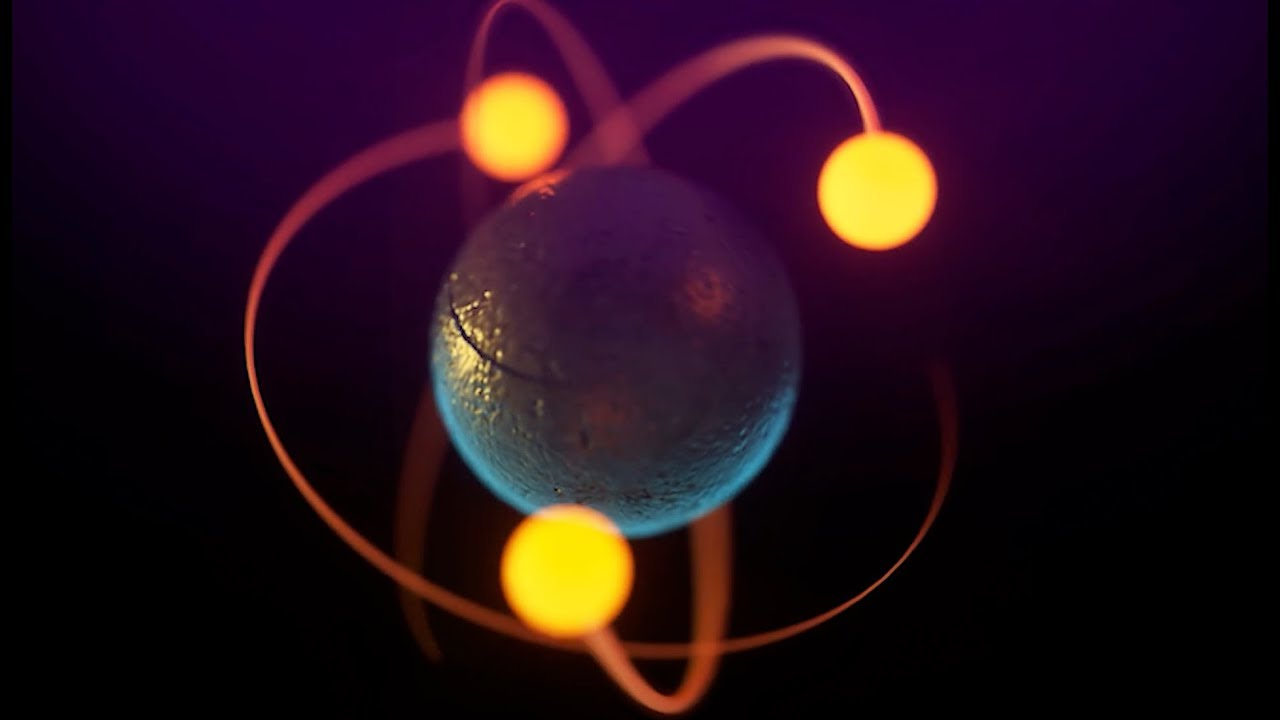
\includegraphics[width=\textwidth,height=\textheight]{figures/back.jpg}};

\node[
color = blue,
align = center,
text width =70cm,
yshift = -5cm,
xshift =  0cm,
anchor = center,
scale=6,
](title) at (current page.north) {A development of a Near-Field Optical Microscope};

\node[anchor = north,
font=\fontsize{35}{42}\selectfont, 
text width=55cm,
inner sep=0pt,
yshift=0cm,
align=center] (author) at (title.south) {\underline{G. A. Mart\'inez-Zepeda$^1$ $^\dagger$},O. Ruiz-Cigarrillo$^1$ $^\ddagger$, K. P. Leija-Alf\'erez$^1$ $^\S$,  L.F. Lastras-Mart\'inez$^1$ $^\ast$.};

\node[font=\fontsize{35}{10}\selectfont, 
text width=55cm,
inner sep=0pt,
anchor = north,
align=center] (places) at (author.south){$^1$ Instituto de Investigaci\'on en Comunicaci\'on \'Optica, Universidad Aut\'onoma de San Luis Potos\'i};
%================================================================%


%LOGOS
\node[anchor=north west,
scale=0.5,
inner sep=0pt,
opacity=1,
](iicologo) at (current page.north west) {
\includegraphics{./figures/Logo_IICO_blue.png}};

\node[anchor=north east,
scale=0.95,
inner sep=0pt,
opacity=1,
](uaslplogo) at (current page.north east) {
\includegraphics{./figures/Logo_UASLP_blue.png}};

\draw[color=blue!90!black, line width=0.25cm](0cm,-15cm)--(90cm,-15cm);
\draw[color=blue!90!black](0cm,-15.5cm)--(90cm,-15.5cm);
%===================================PRINCIPAL BALL=================================%




% PRINCIPAL BALL
% \node [circle,draw, 
%       minimum size=40cm, 
%       line width = \lw,
%       color=black!10!blue, 
%       ball color=black!30!blue,
%       opacity=0.1,
%       yshift = -5cm] (circle1) at (current page.center)  {};

% \node [circle,draw,
%       minimum size=40cm, 
%       line width = \lw,
%       color=black!10!blue,
% opacity=1,
% yshift = -5cm] (circle1) at (current page.center)  {};


\node [ anchor=center,
    minimum size=40cm,
color=black!30!green,
xshift=-1cm,
yshift = -5cm,](im1) at (current page.center) {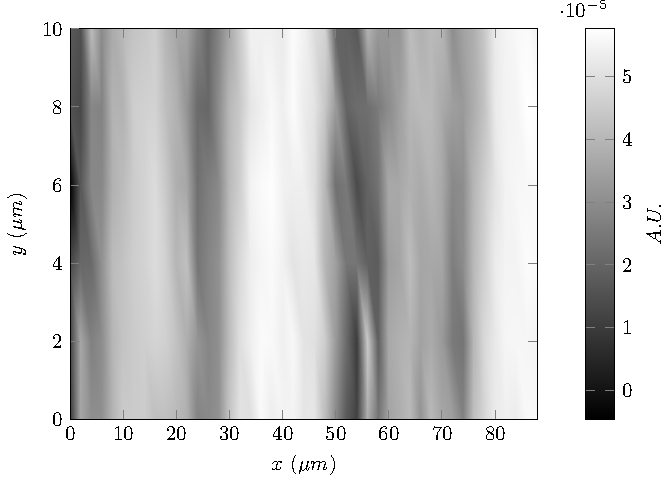
\includegraphics[width=0.4\textwidth]{figures/result/nsomImag/nsomImag.pdf}};

\node [anchor=north,
 text width = 15cm,
 xshift=-10cm, yshift=7cm,
scale=2](t1) at(im1.south east) {NSOM image};




%====================================== Motivacion =================================

\path[draw,
      rounded corners,
      line width = \lw,
      color=black!10!blue] (23.75cm,-57cm) arc  (173:100:21.3cm)--(41.5cm,-38.6cm)--(41.5cm,-18cm)--(31cm,-18cm);


\path[draw,
rounded corners,
line width = \lw,
color=black!10!blue] (14cm,-18cm)--(4cm,-18cm)--(4cm,-57cm)--(23.75cm,-57cm) arc  (173:100:21.3cm);

\node[draw,
rounded corners,
inner sep = 6mm,
line width = \lw,
color = black!10!blue,
font=\bfseries\fontsize{50}{10}\selectfont\color{blue}] at (22.5cm,-18cm) {INTRODUCTION};

\node[anchor=center, 
 xshift = 0cm, 
 align = justify,
 font = \fontsize{37pt}{36}\selectfont, color=blue,
 text width = 35cm] at (22.5cm,-24.5cm) {
	 OBJETIVES
 	\begin{itemize}	
		\item Build a Near-Field Scanning Optical Microscope.
		\item Develop a Control Software in LabVIEW.
		\item Use the NSOM system to observe local optical properties in materials. 
 	\end{itemize}          
 	%\end{tcolorbox}
 };

\node[rotate = 0] (setup) at (15cm,-42cm) {\includegraphics[width=20cm]{figures/systemNSOM.pdf}};
\node[font=\fontsize{24pt}{26.6}\selectfont,yshift =1cm,xshift =10cm,text width = 17cm] at (setup.north west){Figure 1: Optical setup of NSOM};


%\node[anchor=north west,
%xshift=5cm,
%yshift=-20cm,draw](p1) at (current page.north west){\includegraphics[width=0.4\textwidth]{figures/systemNSOM.pdf}};

%\node[anchor=north west,](p2) at (p1.south west){\includegraphics[width=0.4\textwidth]{figures/out/systemNSOM.pdf}};

% \draw (p1.south west) node[name=micrograph]{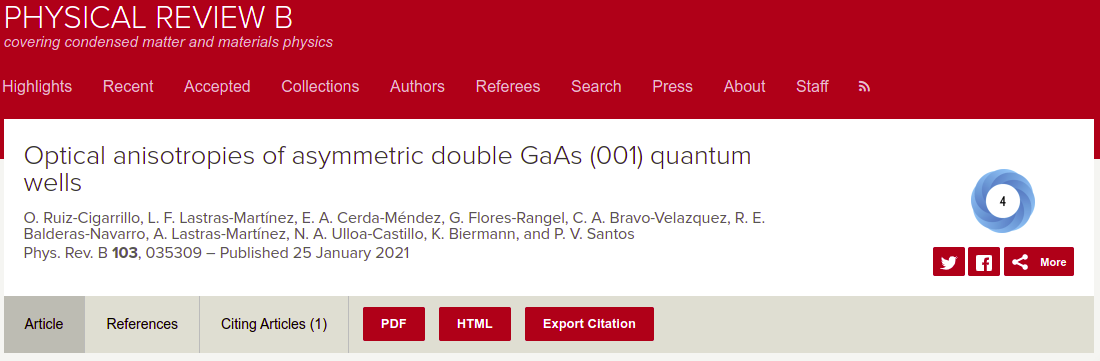
\includegraphics[width=0.4\textwidth]{figures/paper-1.png}};
% \draw[ultra thick, white] (micrograph.south west)++(0.05*0.45\textwidth,0.05*0.45\textwidth)--++(0.45*0.54177\textwidth, 0)node[above,white,midway]{100 \si{\micro\meter}};}


%\node[scale=2,yshift = 0cm,anchor=north west] at (p1.south west){Figure 1: System implemented.};


%============================= OBJETIVOS =====================================%

\path[draw,
      rounded corners,
      line width =\lw,
      color=black!10!blue](66.3cm,-57cm) arc  (7:80:21.3cm) --(48.5cm,-38.6cm)--(48.5cm,-18cm)--(59.7cm,-18cm);
\path[draw,
rounded corners,
line width =\lw,
color=black!10!blue](75.2cm,-18cm)--(86cm,-18cm)--(86cm,-57cm)--(66.3cm,-57cm) arc  (7:80:21.3cm);
      
      
      

\node[draw,
      rounded corners,
	 inner sep = 10mm,
  	 line width = \lw,
     color = black!10!blue,
     font=\bfseries\fontsize{60}{10}\selectfont\color{blue}] at (67.5cm,-18cm) {SAMPLE};


	 \node[rotate = 0] (sample) at (73cm,-35cm) {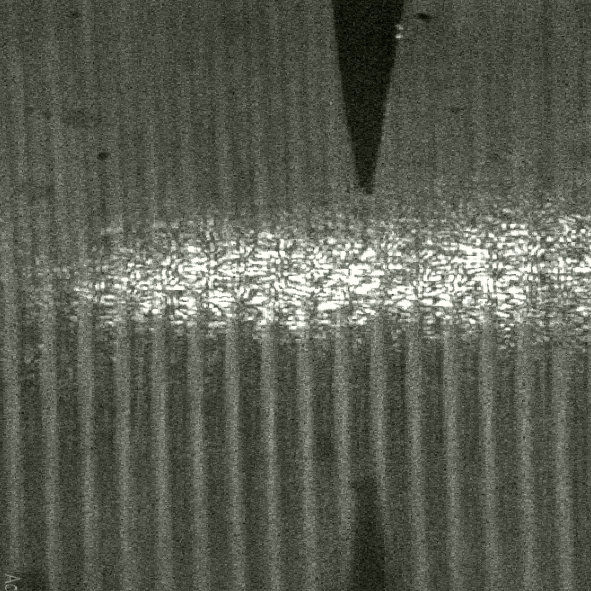
\includegraphics[width=20cm]{figures/tipSample.pdf}};
	 \node[font=\fontsize{24pt}{26.6}\selectfont,yshift =1cm,xshift =10cm,text width = 17cm] at (sample.north west){Figure 2: Tip and Sample Image};
	 

 %\node[anchor=center, 
 %xshift = 0cm, 
 %align = justify,
 %font = \fontsize{30pt}{36}\selectfont, color=blue,
 %text width = 35cm] at (67.5cm,-26.5cm) {
 %	\begin{itemize}	
%		\item Build a Near-Field Scanning Optical Microscope.
%		\item Develop a Control Software in LabVIEW.
%		\item Use the NSOM system to observe local optical properties in materials. 
 %	\end{itemize}          
 %	%\end{tcolorbox}
 %};


%\node[anchor=north east,xshift=-1.5cm,yshift=-18cm](str) at (current page.north east) {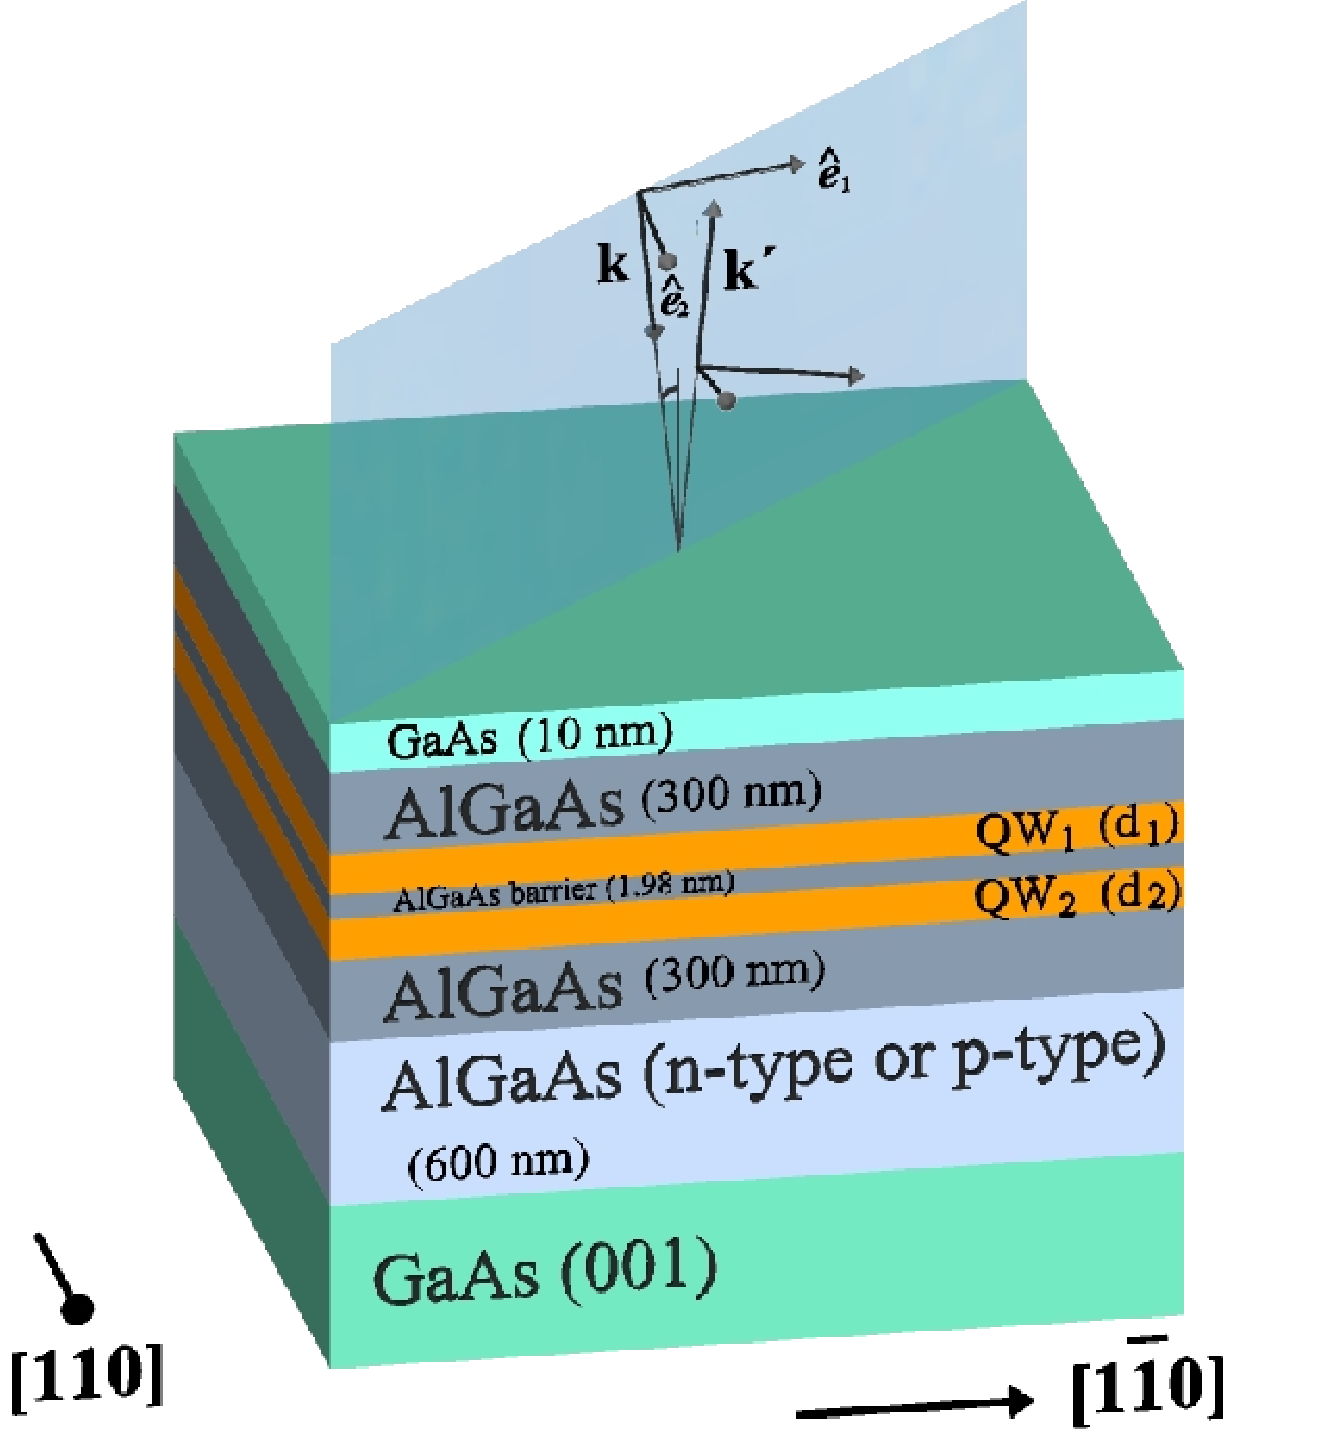
\includegraphics[width=0.3\textwidth]{figures/structure.pdf}};
% \node(DIP) at (76cm,-45cm) {\includegraphics[scale=1.45]{}};

%\node[anchor=north east,
%text width=6cm,scale=2.7, 
%align=justify,
%xshift=1.5cm,
%yshift=-1cm] at (str.north west)
%{In this work, the objective is to start the spin resolve RAS technique in samples of Coupled Quantum Wells, preferentially in the asymmetric samples, which they are possessing a $C_{2v}$ symmetry.};

%\node[anchor=north,scale=2.5,text width = 7cm]
%at (str.south){Figura 2: Sketch of Coupled Quantum Wells structures. };



%========================METODOLOGIA ====================================

\path[draw,
      rounded corners,
      line width = \lw,
      color=black!10!blue] (23.75cm,-59.5cm) arc  (180:225:21cm)-- (30cm,-100cm)--(4cm,-100cm)--(4cm,-59.5cm);
%\path[draw,line width = 0.5cm,color=black!60!green] (24cm,-59.5cm) -- (4cm,-59.5cm)--(4cm,-100cm)--(30cm,-100cm)--(30cm,-74.20cm);
%%\path[draw,line width = 0.5cm] (30.5cm,-75cm) to[bend left] (24cm,-59.5cm);
%\draw[line width = 0.5cm,color=black!60!green] (23.75cm,-59.5cm) arc  (180:225:21cm);



\node[draw,
	  rounded corners,
	  inner sep = 2.5mm,
	  line width = \lw,
	  color = black!10!blue,
      scale=4.5,
	  color=blue,
	  font=\bfseries] at (13.85cm,-60cm) {Topographic};


%\node[anchor=north,
%red,
%scale=2.8] (ft) at (13.85cm,-63cm) {Reflectance Anisotropy Spectroscopy};

%\node[anchor = north,
%font = \fontsize{30pt}{36}\selectfont,
%yshift = 0cm,
%align = justify,
%text width = 20cm](ftt) at (ft.south){
%	\begin{itemize}
%	 \item The setup conssit in a l.
%	 \item The aim of this work, it's purpose the way to carried RAS experiments to do it spin sensitive. 
%	 \item As first approximation, we purpose measured it trough two polarization states with the photo-elastic modulator device. 
%	\end{itemize}
%};



%\node at (23cm,-85cm) {\includegraphics[scale=1]{./FIGURES/Sample/Sample-1}};

\node[rotate = 0] (topo1) at (15cm,-75cm) {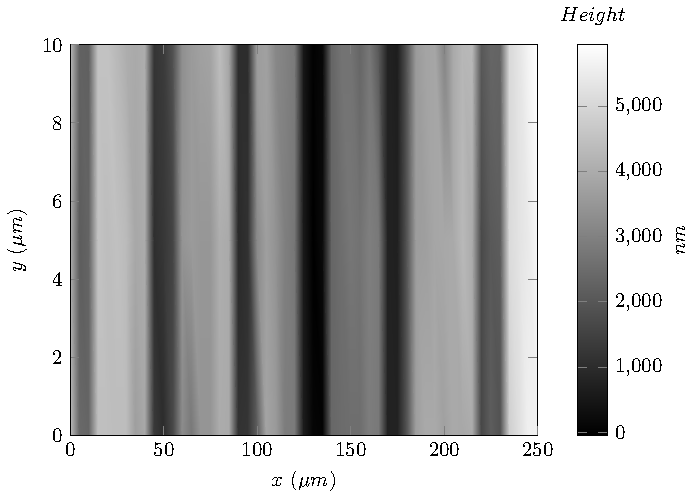
\includegraphics[width=20cm]{figures/result/extafmImag/exAFMImag.pdf}};
\node[font=\fontsize{24pt}{26.6}\selectfont,yshift =1cm,xshift =10cm,text width = 17cm] at (topo1.north west){Figure 3: Topographic image of InP Grating in a region of $250 \times 10 ~ \mu m$.};

\node[rotate = 0] (topo2) at (15cm,-93cm) {\includegraphics[width=20cm]{figures/result/afmImag/AFMImag.pdf}};
\node[font=\fontsize{24pt}{26.6}\selectfont,yshift =1cm,xshift =10cm,text width = 17cm] at (topo2.north west){Figure 4: Topographic image of InP Grating in a region of $88 \times 10 ~ \mu m$.};



%==================== CONCLUSIONES =================================================%


\path[draw,
      rounded corners,
      line width = \lw,
      color=black!10!blue] 
([shift={(45cm,-62cm)}]240:19cm) arc[radius=19cm, start angle=240, end angle= 300]--(56cm,-81cm) arc(300:240:22cm)--cycle;


\path[draw,
rounded corners,
line width = \lw,
color=black!10!blue] (55.5cm,-80cm)--(56cm,-79.5cm)--(58cm,-79.5cm)--(58cm,-100cm)--(32cm,-100cm)--(32cm,-79.5cm)--(34cm,-79.5cm)--(34.5cm,-80cm);


\def\myshift#1{\raisebox{-1.75ex}}
\draw[draw=none,
      blue,
      postaction={decorate},
      decoration={text along path,text={|\bfseries\fontsize{60}{10}\selectfont\color{blue}\myshift|CONCLUSIONS},text align=center}]
([shift={(45cm,-64.85cm)}]240:17cm) arc [start angle=240,end angle=300,radius=17cm];

 \node[font = \fontsize{30pt}{36}\selectfont,
 align = justify,
 color =blue,
text width = 25cm]  at (45cm, -91.75cm) {
 	\begin{itemize}	
	     \item An automation software capable of performing simultaneous topographic and near field measurements was developed usign LabVIEW used to adquire the topographic and NSOM image.
         \item The first result show interesting properties and guive information about the local optical properties. 
    
 \end{itemize}

 };





%===================================== RESULTADOS ==================================%

\path[draw,
      rounded corners,
      line width = \lw,
      color=black!10!blue] (60cm,-74.5cm)  arc  (-45:0:21cm)--(70cm,-59.5cm);
\draw[draw,
      rounded corners,
      line width =\lw,
      color = black!10!blue] (82cm,-59.5cm)--(86cm,-59.5cm)--(86cm,-100cm)--(60cm,-100cm)--(60cm,-74.5cm);

%\path[draw,line width = 0.5cm,color=black!60!green] (66cm,-59.5cm) -- (86cm,-59.5cm)--(86cm,-100cm)--(60.5cm,-100cm)--(60cm,-74.20cm);
%%\path[draw,line width = 0.5cm,color=black!60!green] (60cm,-74.5cm) to[bend right](66cm,-59.5cm);
%
%\draw[line width = 0.5cm,color=black!60!green] (60cm,-74.5cm)  arc  (-45:0:21cm);

\node[draw,
      rounded corners,
      inner sep = 2.5mm,
      line width = \lw,
      color = black!10!blue,
     scale=4.5,
	 font=\bfseries](RESUL) at (76cm,-59.5cm) {RESULTS};





\node[anchor=south east,xshift=-5cm,yshift=10cm](RAS) at (90cm,-103cm){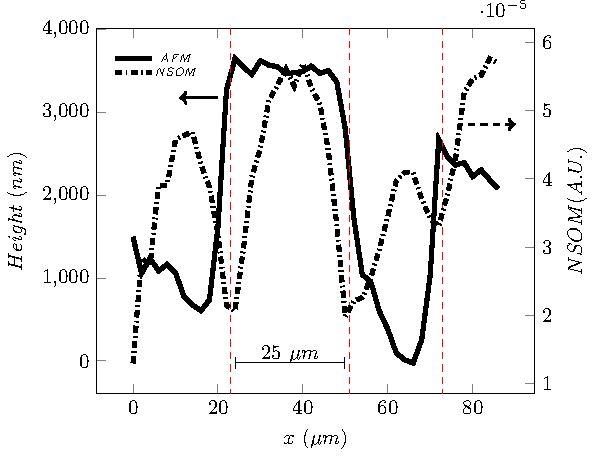
\includegraphics[width=0.26\textwidth]
	{figures/result/compProf/compafmnsom.pdf}};
	\node[font=\fontsize{24pt}{26.6}\selectfont,yshift =1cm,xshift =10cm,text width = 17cm] at (RAS.north west){Figure 5: Comparison bewteen profiles of topographical and NSOM measurements.};

% \node[anchor = north,
% font = \fontsize{18pt}{21.6}\selectfont,
% yshift =-0cm,
% xshift = 0cm,
% align = justify,
% text width = 24cm
% ](tf3) at (PR.south) {Figura 6: (a)  C\'alculo de las energ\'ias y las funciones de onda correspondientes para la estructura estudiada.
% 	(b) Espectros de Fotorreflectancia medidos a diferentes potencias del l\'aser, en los cuales se puede observar la evoluci\'on del TRION conforme se aumenta la potencia. Otro aspecto interesante es la transici\'on indirecta alrededor de 822nm.  };



%
%\node[anchor = west,
%font = \fontsize{18pt}{21.6}\selectfont,
%align = justify,
%text width = 8cm,
%yshift = -2.5cm] at(QW1.north east){Figura 5: C\'alculo de las energ\'ias y las funciones de onda correspondientes para la estructura estudiada.};



%==================================================================%





% REFERENCES




\node[draw,
rounded corners,
font=\fontsize{20pt}{15}\selectfont, 
line width =\lw,
color=black!10!blue,
inner sep =0.35cm]at (45cm,-104.25cm) {\parbox{81.5cm}{
		 \bibliography{posterBiblio}}};


\draw[fill = black] (0cm,-108cm)--(90cm,-108cm)--(90cm,-110cm)--(0cm,-110cm)--(0cm,-108cm);



\node[white,font=\bfseries\fontsize{25pt}{15}\selectfont] at (10cm,-109cm) {gabmtzz27@gmail.com$^\dagger$};
\node[white,font=\bfseries\fontsize{25pt}{15}\selectfont] at (35cm,-109cm) {oscarruiz@cactus.iico.uaslp.mx$^\ddagger$};
\node[white,font=\bfseries\fontsize{25pt}{15}\selectfont] at (55cm,-109cm) {a236792@alumnos.uaslp.mx$^\S$};
\node[white,font=\bfseries\fontsize{25pt}{15}\selectfont] at (80cm,-109cm) {lflm@cactus.iico.uaslp.mx$^\ast$};
%==================================================================%






%DIBUJAR FLECHAS
%\path[draw,myarrow,shorten <= -0.5cm, shorten >= -0.5cm] (circle1) to (circle2);


%==================================================================%



\end{tikzpicture}

\end{document}